\scanpage{113}

\figure{%
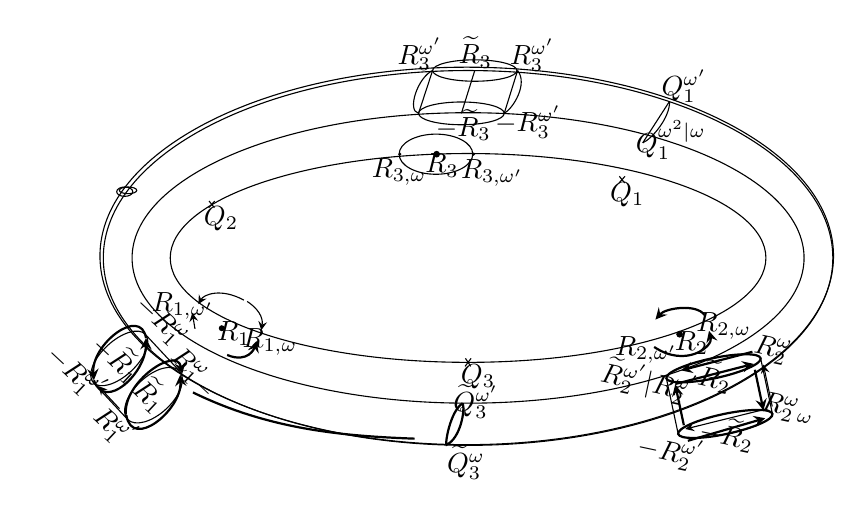
\begin{tikzpicture}[x=0.85cm,y=0.85cm,>=stealth]
\draw[thin] (0,0) ellipse (5.45 and 2.8);
\draw[thin] (-0.02,0.03) ellipse (5.48 and 2.82);
\draw[thin] (0,0) ellipse (5.02 and 2.17);
\draw[thin] (0,0) ellipse (4.45 and 1.56);
\draw[thick] (-4.11,-2.01) .. controls (-2.98,-2.56) and (-1.9,-2.66) .. (-0.8,-2.7);
\fill (-0.47,1.55) circle (0.05);\node at (-0.39,1.38) {$R_3$};
\draw[thin] (-0.48,1.55) ellipse (0.55 and 0.3);
\fill (-1.02,1.55) circle (0.025);\fill (0.08,1.55) circle (0.025);
\node at (-1.03,1.28) {$R_{3,\omega}$};\node at (0.36,1.27) {$R_{3,\omega'}$};
\draw[thin] (0.1,2.8) ellipse (0.63 and 0.16);
\draw[thin] (-0.1,2.16) ellipse (0.64 and 0.17);
\draw[thin] (-0.53,2.8) -- (-0.74,2.16);\draw[thin] (0.74,2.8) -- (0.54,2.16);
\draw[thin] (0.1,2.8) -- (-0.1,2.16);
\draw[thin] (-0.53,2.8) .. controls (-0.75,2.7) and (-0.92,2.2) .. (-0.74,2.16);
\draw[thin] (0.74,2.8) .. controls (0.9,2.6) and (0.67,2.23) .. (0.54,2.16);
\node at (0.11,3.07) {$\widetilde{R}_3$};\node at (-0.07,1.99) {$-\widetilde{R}_3$};
\node at (-0.72,3.04) {$\unsure{R_3^{\omega'}}$};\node at (0.96,3.03) {$\unsure{R_3^{\omega'}}$};
\node at (0.9,2.03) {$-R_3^{\omega'}$};
\draw[thin] (3.01,2.34) .. controls (3.02,2.1) and (2.75,1.78) .. (2.61,1.72);
\draw[thin] (3.01,2.34) -- (2.61,1.72);
\node at (3.23,2.57) {$Q_1^{\omega'}$};\node at (3.03,1.76) {$Q_1^{\unsure{\omega^2|\omega}}$};
\draw (2.3,1.17) ++(-0.045,-0.05) -- ++(0.09,0.1);\draw (2.3,1.17) ++(-0.04,0.05) -- ++(0.08,-0.1);
\node at (2.38,0.95) {$Q_1$};
\draw (-3.83,0.8) ++(-0.045,-0.05) -- ++(0.09,0.1);\draw (-3.83,0.8) ++(-0.04,0.05) -- ++(0.08,-0.1);
\node at (-3.69,0.59) {$Q_2$};
\draw[thin] (-5.08,1.01) ellipse (0.13 and 0.05);
\draw[thin] (-5.13,0.99) ellipse (0.12 and 0.07);
\draw (0,-1.56) ++(-0.045,-0.06) -- ++(0.09,0.12);\draw (0,-1.56) ++(-0.04,0.06) -- ++(0.08,-0.12);
\node at (0.15,-1.78) {$Q_3$};
\draw[thick] (-0.08,-2.17) .. controls (-0.27,-2.29) and (-0.35,-2.79) .. (-0.32,-2.79) .. controls (-0.12,-2.7) and (-0.04,-2.28) .. (-0.08,-2.17);
\node at (0.12,-2.15) {$\widetilde{Q}_3^{\omega'}$};\node at (-0.03,-3.06) {$\unsure{\widetilde{Q}_3^{\omega}}$};
\begin{scope}[shift={(-3.68,-1.05)}]
\fill (0,0) circle (0.045);\node at (0.18,-0.08) {$R_1$};
\draw[->] (0.33,0.42) .. controls (-0.02,0.61) and (-0.27,0.5) .. (-0.35,0.36);
\draw[->] (0.38,0.4) .. controls (0.62,0.24) and (0.61,0.09) .. (0.59,-0.03);
\draw[->,thick] (0.08,-0.4) .. controls (0.4,-0.53) and (0.49,-0.29) .. (0.52,-0.19);
\draw[->] (-0.4,-0.01) -- (-0.44,0.23);
\node at (-0.58,0.33) {$R_{1,\omega'}$};\node at (0.72,-0.21) {$R_{1,\omega}$};
\end{scope}
\begin{scope}[shift={(-4.7,-2.05)},rotate=43]
\draw[thin] (0,0) ellipse (0.53 and 0.28);\draw[thin] (0,0.75) ellipse (0.53 and 0.26);
\draw[thin] (-0.53,0) -- (-0.53,0.75);\draw[thin] (0.53,0) -- (0.53,0.75);
\draw[->,thick] (-0.5,0.06) .. controls (-0.8,-0.39) and (0.16,-0.45) .. (0.5,-0.05);
\draw[->,thick] (-0.5,0.07) .. controls (-0.19,0.46) and (0.76,0.3) .. (0.53,-0.06);
\draw[->,thick] (-0.5,0.77) .. controls (-0.7,0.31) and (0.14,0.32) .. (0.5,0.7);
\draw[->,thick] (0.5,0.7) .. controls (0.77,1.11) and (-0.17,1.19) .. (-0.5,0.77);
\draw[->] (-0.51,0.2) -- (-0.51,0.66);
\node[rotate=-43] at (-0.02,0.03) {$\widetilde{R}_1$};\node[rotate=-43] at (0,0.77) {$-\widetilde{R}_1$};
\node[rotate=-43] at (-0.74,0.05) {$R_1^{\omega'}$};\node[rotate=-43] at (0.67,-0.18) {$R_1^\omega{}_{\deleted{\unsure{-}}}$};
\node[rotate=-43] at (-0.61,1.04) {$-R_1^{\omega'}$};\node[rotate=-43] at (0.82,0.73) {$-R_1^\omega$};
\end{scope}
\begin{scope}[shift={(3.16,-1.14)}]
\fill (0,0) circle (0.05);\node at (0.18,-0.13) {$R_2$};
\draw[->,thick] (0.37,0.29) .. controls (0.25,0.46) and (-0.21,0.39) .. (-0.36,0.22);
\draw[->,thick] (-0.38,-0.19) .. controls (0.1,-0.51) and (0.5,-0.18) .. (0.44,0.05);
\node at (-0.5,-0.23) {$R_{2,\omega'}$};\node at (0.66,0.12) {$R_{2,\omega}$};
\end{scope}
\begin{scope}[shift={(3.75,-2.04)},rotate=12]
\draw[thick] (0,0.4) ellipse (0.72 and 0.15);\draw[thick] (0,-0.45) ellipse (0.72 and 0.15);
\draw (-0.72,0.4) -- (-0.72,-0.45);\draw (0.72,0.4) -- (0.72,-0.45);
\draw[->,thick] (0.62,0.52) -- (-0.48,0.47);\draw[->,thick] (-0.6,0.29) -- (0.6,0.34);
\draw[->,thick] (0.6,0.25) -- (0.6,-0.37);\draw[->] (0.74,-0.34) -- (0.74,0.3);
\draw[->,thick] (-0.61,-0.34) -- (-0.61,0.28);
\draw[->,thick] (-0.6,-0.58) -- (0.6,-0.49);\draw[->] (0.6,-0.36) -- (-0.6,-0.4);
\node[rotate=-12] at (0,0.27) {$\widetilde{R}_2$};\node[rotate=-12] at (0,-0.59) {$-\widetilde{R}_2$};
\node[rotate=-12] at (-0.98,0.4) {$\unsure{\widetilde{R}_2^{\omega'}|R_2^{\omega'}}$};
\node[rotate=-12] at (0.92,0.48) {$R_2^\omega$};
\node[rotate=-12] at (-0.88,-0.68) {$-R_2^{\omega'}$};
\node[rotate=-12] at (0.96,-0.43) {$R_2^\omega{}_{\deleted{\unsure{\omega}}}$};
\end{scope}
\end{tikzpicture}%
}

\figure{%
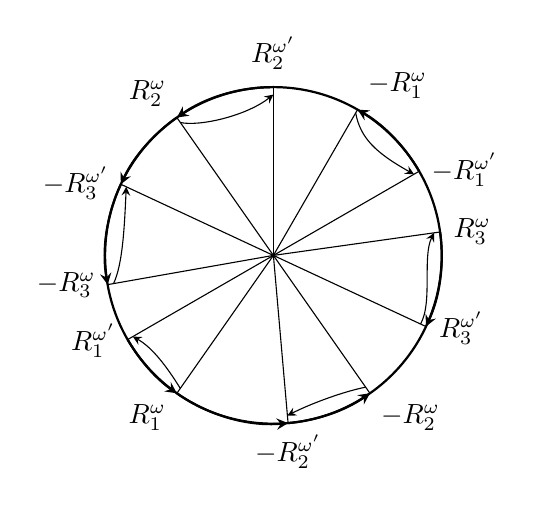
\begin{tikzpicture}[x=0.95cm,y=0.95cm,>=stealth]
\draw[thick] (0,0) circle (2.25);
\foreach \a in {90,125,60,30,8,-25,-55,-85,-125,-150,-170,155}{\draw[thin] (0,0)--(\a:2.25);}
\node[above] at (90:2.35) {$R_2^{\omega'}$};
\node[above left] at (125:2.27) {$R_2^\omega$};
\node[above right] at (60:2.27) {$-R_1^\omega$};
\node[right] at (30:2.29) {$-R_1^{\omega'}$};
\node[right] at (8:2.3) {$R_3^\omega$};
\node[right] at (-25:2.3) {$R_3^{\omega'}$};
\node[below right] at (-55:2.28) {$-R_2^\omega$};
\node[below] at (-85:2.28) {$-R_2^{\omega'}$};
\node[below left] at (-125:2.28) {$R_1^\omega$};
\node[left] at (-150:2.28) {$R_1^{\omega'}$};
\node[left] at (-170:2.28) {$-R_3^\omega$};
\node[left] at (155:2.28) {$-R_3^{\omega'}$};
\draw[->,thick] (90:2.25) arc (90:125:2.25);
\draw[->] (125:2.17) .. controls (-1.0,1.72) and (-0.37,1.86) .. (90:2.15);
\draw[->,thick] (125:2.25) arc (125:155:2.25);
\draw[->] (60:2.2) .. controls (1.16,1.57) and (1.37,1.37) .. (30:2.17);
\draw[->,thick] (30:2.25) arc (30:60:2.25);
\draw[->,thick] (8:2.25) arc (8:-25:2.25);
\draw[->] (-25:2.17) .. controls (2.13,-0.64) and (1.99,-0.01) .. (8:2.17);
\draw[->,thick] (-85:2.25) arc (-85:-55:2.25);
\draw[->] (-55:2.15) .. controls (0.89,-1.83) and (0.44,-2.01) .. (-85:2.15);
\draw[->,thick] (-125:2.25) arc (-125:-85:2.25);
\draw[->,thick] (-150:2.25) arc (-150:-125:2.25);
\draw[->] (-125:2.17) .. controls (-1.43,-1.48) and (-1.62,-1.23) .. (-150:2.17);
\draw[->,thick] (155:2.25) arc (155:190:2.25);
\draw[->] (-170:2.17) .. controls (-2.01,-0.11) and (-1.99,0.43) .. (155:2.17);
\end{tikzpicture}%
}

$P_i^{\omega,\zeta}$ prend $12$ valeurs distinctes

\unsure{pq|puis} six valeurs pour \deleted{$\unsure{P_i^\omega}$} $\zeta$ fixé (les $P_i^\omega$) et les six

\figure{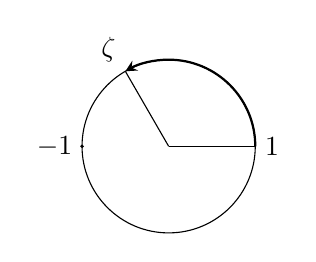
\begin{tikzpicture}[>=stealth]
\draw (0,0) circle (1.1);
\draw (0,0)--(1.1,0);\draw (0,0)--(120:1.1);
\draw[->,thick] (1.1,0) arc (0:120:1.1);
\fill (-1.1,0) circle (0.025);\node[left] at (-1.1,0) {$-1$};
\node[right] at (1.1,0) {$1$};\node[above left] at (120:1.1) {$\zeta$};
\end{tikzpicture}}

\[
Q_i^\omega=R_j-R_k\longmapsto R_j-\zeta R_k
=P_i^{\omega\deleted{\unsure{\zeta}}}=P_i^{\omega,\zeta}
\]
\[
P_i^{\omega,\zeta}=R_{\omega i}\deleted{\unsure{\zeta}}-\zeta R_{\omega^{\unsure{2|4}}i}
\qquad=-P_{\omega^2i}^{\omega,\zeta}
\]
\[
P_i^{\omega',\zeta'}=R_{\omega'i}-\zeta'R_{\omega i}
=R_k-\zeta^2R_j=-\zeta'P_i^{\omega,\zeta}
\]

\mspage{112}
